\documentclass[a4paper]{article}

% Language setting
% Replace `english' with e.g. `spanish' to change the document language
\usepackage[english]{babel}

% Useful packages
\usepackage{amsmath}
\usepackage{amsfonts}
\usepackage{graphicx}
\usepackage[inkscapelatex=false]{svg}
\usepackage{float}
\usepackage{listings}
\usepackage{subcaption}
\usepackage{xcolor}
\usepackage[colorlinks=false]{hyperref}

\definecolor{codegreen}{rgb}{0,0.6,0}
\definecolor{codegray}{rgb}{0.5,0.5,0.5}
\definecolor{codepurple}{rgb}{0.58,0,0.82}
\definecolor{backcolour}{rgb}{0.95,0.95,0.92}
\lstdefinestyle{mystyle}{
    backgroundcolor=\color{backcolour},
    commentstyle=\color{codegreen},
    keywordstyle=\color{magenta},
    numberstyle=\tiny\color{codegray},
    stringstyle=\color{codepurple},
    basicstyle=\ttfamily,
    breakatwhitespace=false,         
    breaklines=true,                 
    captionpos=b,                    
    keepspaces=true,                 
    numbers=left,                    
    numbersep=5pt,                  
    showspaces=false,                
    showstringspaces=false,
    showtabs=false,                  
    tabsize=2,
    xleftmargin=0.01\textwidth,
    escapeinside={(*@}{@*)},
}
\lstset{style=mystyle}

\newcommand{\ccvmn}{\lstinline{concaveman}}

\newcommand{\cctd}{\lstinline{concaveman3d}}

\title{The ``concaveman'' package,\\analysis and expansion}
\author{Bruniera Alvise (142491) \and Cavasin Riccardo (144692)}

\begin{document}
\maketitle

\begin{abstract}
The ``\ccvmn'' \cite{10.32614/CRAN.package.concaveman} CRAN package offers the the ``\ccvmn'' javascript package (\url{https://github.com/mapbox/concaveman}) in R, to efficiently compute the 2D concave hull.

The algorithm used in \ccvmn~improves over the algorithm developed by Jin-Seo Park and Se-Jong Oh \cite{Park2012ANC}, which can be generalized to $n$ dimensions, with better performance.

Despite the algorithm being designed for $n$ dimensions, the implementation in ``\ccvmn`` only supports points in a 2D space.

We will provide a 3-dimensional implementation, and then we will find that the algorithm, as it is presented in the paper, can not actually produce useful results in 3D spaces.
\end{abstract}

\tableofcontents

\newpage

\section{Introduction}

A ``hull`` is a polyhedron that fully encloses a cloud of points. The most frequently encountered kind of hull is the ``convex hull'', which is the minimal convex polyhedron that fully encloses a cloud of points. Efficient algorithm for computing the convex hull in $n$ dimensions are available, with complexity as low as $O(n\log n)$ \cite{10.1145/235815.235821}.

The ``concave hull'' is a concave polyhedron that fully encloses a cloud of points, and is itself enclosed within the convex hull. Unlike the convex hull, minimality can be undesired, as a minimal concave hull would likely have jagged, extreme shapes. Instead we require the concave hull to not be bigger than the convex hull, and provide a smoothness parameter to adjust the result.

The purpose of a concave hull in statistical analysis is to represent more closely clustering information, that cannot be faithfully represented by a convex hull.

\begin{figure}[H]
    \centerline{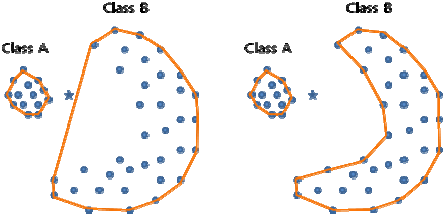
\includegraphics[width=0.8\columnwidth]{4.png}}
    \caption{A concave hull does a better job of capturing cluster $B$}
    \label{fig:cluster}
\end{figure}

As shown in Figure \ref{fig:cluster}, in some datasets, clusters have large empty areas. Summarising the clusters with a convex hull might lead to mis-categorization of new data, when it is close to an edge of the convex hull, but not to the actual cluster of datapoints.
In this case, a concave hull will match the cluster's shape more faithfully, allowing to better recognize new datapoints.

\subsection{Prior art}

This algorithm poses itself as both efficient and $n$ dimensional-capable algorithm, in contrast with previous known algorithms which compromised on generality:

\begin{description}
    \item Swing arm\cite{10.1007/11863939_6}
    \begin{itemize}
        \item Can be extended to $n$ dimensions
        \item Has complexity $O(n^3)$
    \end{itemize}
    \item $\chi$-shape\cite{10.1016/j.patcog.2008.03.023}
    \begin{itemize}
        \item Can be extended to $n$ dimensions
        \item Has complexity $O(n^3)$
    \end{itemize}
    \item KNN-based approach\cite{10.1145/2505821.2505827}
    \begin{itemize}
        \item Has complexity $O(n\log n)$
        \item Cannot be extended to $n$ dimensions
    \end{itemize}
    \item ``Park-Oh'' algorithm
    \begin{itemize}
        \item Has complexity $O(n\log n+rn)$ where $r$ is the number of points in the output hull
        \item Can easily be extended to $n$ dimensions
        \item The complexity is further reduced to $O(n\log n)$ by ``\ccvmn''
    \end{itemize}
\end{description}

\section{Concave hull algorithm}

\subsection{Overview}

We will describe the two dimensional version of the algorithm, and then show how it can be extended to any dimension. The algorithm proceeds in four phases:

\begin{enumerate}
    \item The convex hull is computed with a known algorithm, and a threshold value $N$ is obtained from the smoothness parameter.
    \item Then the nearest inner points to every edge are found, and the distance between the inner point and the nearest vertex of the edge is computed (called decision distance).
    \item If the ratio between edge length and decision distance is greater than $N$, the edge is ``dug'' (the edge is removed and two new edges are added between the ex-inner-point and the old edge vertices).
    \item The second and third steps are repeated until there are no edges to dig.
\end{enumerate}

\subsection{Definitions}

\begin{description}
    \item $G=\{p_1,...,p_n\}\subseteq\mathbb R^m$ is a set of points in an $m$-dimensional space, which is the input of the algorithm
    \item $N\in\mathbb R^+$ is a non-negative real number which is a measure of smoothness, which can be fixed or given as input to the algorithm
    \item $ConvexList(G)\subseteq \mathbb R^{mm}$ is the (unordered) set of facets that constitutes the convex hull of $G$ (edges in the 2-dimensional case, and triangles in the 3-dimensional case)
    \item $D(p_1,p_2)$ is the distance between two points
    \item $DD(p,Q)$ with $Q\subseteq\mathbb R^m$ is the ``decision distance'' (Figure \ref{fig:dd}) between point $p$ and set of points $Q$, defined as:
    $$DD(p,Q)=\min\{D(p,q_i)|q_i\in Q\}$$
    \item $DE(p,(e_1,e_2)$ is the distance between the point $p$ and edge $(e_1,e_2)$, defined as:
    $$DE(p,(e_1,e_2))=\min\{D(p,e_i)|e_1\mathrm{~is~a~point~along~}(e_1,e_2)\}$$
    \item $DT(p,(t_1,t_2,t_3)$ is the distance between the point $p$ and triangle $(t_1,t_2,t_3)$, defined as:
    $$DT(p,(t_1,t_2,t_3))=\min\{D(p,t_i)|t_1\mathrm{~is~a~point~in~}(t_1,t_2,t_3)\}$$
    \item More generally, we can define $DM(p,(p_1,...,p_m))$ as the distance between point $p$ and an $m$-dimensional facet $(p_1,...,p_m)$
\end{description}

\begin{figure}[H]
    \centerline{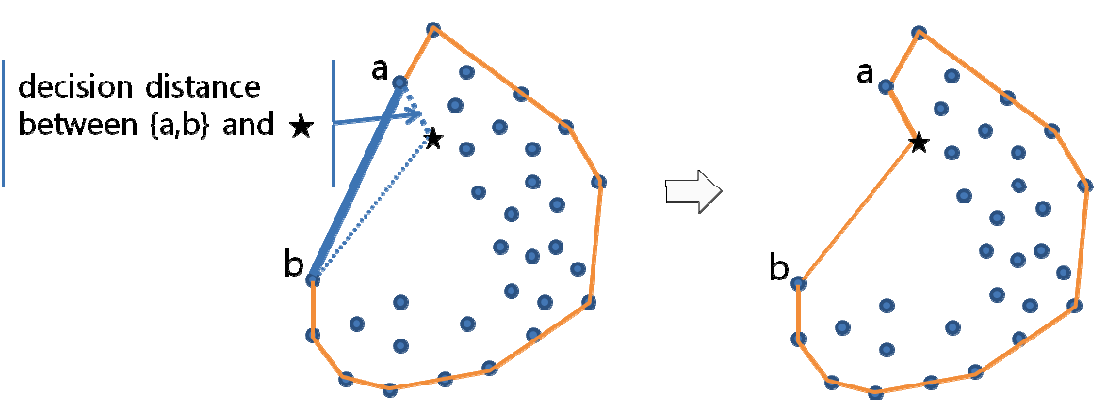
\includegraphics[width=0.8\columnwidth]{dd.png}}
    \caption{Digging process and decision distance}
    \label{fig:dd}
\end{figure}

\subsection{Pseudocode}

We present the pseudocode for the algorithm in 2-dimensional space:

\begin{lstlisting}[language=c]
/**
Input: G // target dataset
Output: ConcaveList // set of edges that forms a 2 dimensional concave hull
**/

function ConcaveHull(G) {
    ConvexHull = ConvexList(G); // using a known algorithm
    choose N; // given as input or fixed
    /* 2. Digging convex */
    ConcaveList = ConvexHull;
    for i = 1 to the end of the ConcaveList  {
        E = ConcaveList[i]
        P_k = find P_k such that:
            DE(P_k, E) is minimal &&
            forall E_a adjacent to E:
                DE(P_k, E_a) >= DE(P_k, E);
        
        eh = D(E[1], E[2]); // the length of the edge
        dd = DD(P_k, E);
        if (eh/dd) > N { // digging process
            ConcaveList.add([E[1], P_k]);
            ConcaveList.add([P_k, E[2]]);
            ConcaveList.delete(E);
        }
    }
    return ConcaveList;
}
\end{lstlisting}

The same algorithm can easily be modified to work in three dimensions, or even $m$ dimensions; we just need to use the appropriate $DM()$ to calculate the distance and a reasonable measure of facet size.
We define the algorithm for the 3-dimensional case as:

\begin{lstlisting}[language=c]
/**
Input: G // target dataset
Output: ConcaveList // set of triangles that forms a 3 dimensional concave hull
**/

function ConcaveHull(G) {
    ConvexHull = ConvexList(G); // using a known algorithm
    choose N; // given as input or fixed
    /* 2. Digging convex */
    ConcaveList = ConvexHull;
    for i = 1 to the end of the ConcaveList  {
        T = ConcaveList[i]
        P_k = find P_k such that:
            DT(P_k, T) is minimal &&
            forall T_a adjacent to T:
                DT(P_k, T_a) >= DT(P_k, T);
        
        th = (D(E[1], E[2]) + D(E[2], E[3]) + D(E[3], E[1]))/3;
        // the size of the triangle
        dd = DD(P_k, E);
        if (th/dd) > N { // digging process
            ConcaveList.add([E[1], E[2], P_k]);
            ConcaveList.add([E[2], E[3], P_k]);
            ConcaveList.add([E[3], E[1], P_k]);
            ConcaveList.delete(E);
        }
    }
    return ConcaveList;
}
\end{lstlisting}

\subsection{Complexity}

The most critical part of the algorithm is finding the point $p_k$ that is the closest to facet $e$, but not closer to an adjacent facet of $e$.
In the 2-dimensional case, the adjacent edges are always two, so the complexity of checking the distance to the adjacent edges is $O(1)$. Thus, as stated in the paper, the complexity is $O(rn)$ where $n$ are points in the input, and $r$ the vertices of the hull. Combined with the convex hull complexity, the total cost amounts to $O(n\log n+rn)$. Interestingly, the shape of the hull affects performance.

In the 3-dimensional (or $n$-dimensional) case, this does not hold, because a triangle can have arbitrarily many adjacent triangles. As such, for every candidate point, verifying that it is not closer to an adjacent triangle has cost $O(n)$, for a total of $O(rn^2)$. This is in contradiction with the paper, which states that increasing dimensionality should increase the time complexity by some additive constant.

To achieve the stated complexity, we would need an algorithm to compute efficiently the nearest points, but the paper doesn't provide one.
\ccvmn~ accelerates the search with a customized version of the K-Nearest algorithm, but we choose to focus on the paper's version.

\subsection{Incorrectness of the algorithm}\label{sub:incorrectness}

The algorithm as presented cannot work in 3 dimensions. We will discuss two main criticalities:

\bigskip

The algorithm only digs on faces, leaving edges unchanged, and creates new edges to repair the surface. This flaw makes it impossible to wrap correctly almost every concave point cloud, resulting in extra edges covering big gaps, like in Figure \ref{fig:chair}, or ``sponge-like'' shapes, like in Figure \ref{fig:cube} and Figure \ref{fig:cup}. This behaviour makes the algorithm fundamentally useless for statistical analysis.

\begin{figure}[H]
    \begin{subfigure}{.5\textwidth}
        \centerline{\includegraphics[height=5.5cm]{chair2.png}}
        \caption{3D model of a chair: Faces are dug between the seat and backrest, leaving the edges on the side and the diagonal}
        \label{fig:chair}
    \end{subfigure}
    \begin{subfigure}{.5\textwidth}
        \centerline{\includegraphics[height=5.5cm]{cube.png}}
        \caption{Random points in a cube: Faces are dug in forming deep narrow caves}
        \label{fig:cube}
    \end{subfigure}
    \centerline{\begin{subfigure}{.7\textwidth}
        \includegraphics[height=5.5cm]{cup.png}
        \caption{3D model of a cup: The faces around the handle have been dug,but without revealing the handle, due to the edges}
        \label{fig:cup}
    \end{subfigure}}
    \caption{3D point concave hulls showing the ``caving'' behaviour of the algorithm}
    \label{fig:caving}
\end{figure}

\bigskip

The second criticality is a fundamental incorrectness in the idea behind the algorithm. The algorithm checks that the candidate ``digging point'' is not closer to some adjacent facet than it is to the facet being analysed, in order to avoid creating self-intersections.

This works in 2D when considering a convex shape, but doesn't once the shape has been made concave, although, one can work around this issue by checking the distance from all edges instead of just adjacent edges (rising the complexity), or by utilizing a more sophisticated data structure to find the candidate points (like \ccvmn~ does).

In 3D this issue is even more prominent. Even if we were to check the distance from all edges, there is still the possibility that a new triangle intersects another. We can see an instance of this edge case in Figure \ref{fig:degenerate-triangles}.
The only way to catch this behaviour would be checking each face for interception (costly), or by choosing a higher smoothness value ($N$) in a case by case basis, so that there's barely any digging made.

Together, these issues yield overall poor results, as the intersecting edge will never be removed and new edges incident to it will be intersecting.

Both of these flaws are inherent to the design of the algorithm and render it unsuitable for 3-dimensional spaces.

\begin{figure}[H]
    \begin{subfigure}{.5\textwidth}
        \centerline{\includegraphics[height=5cm]{crossing-triangles.pdf}}
        \caption{Diagram of the problematic triangles and points arrangement}
    \end{subfigure}
    \begin{subfigure}{.5\textwidth}
        \centerline{\includegraphics[height=5cm]{triangles.png}}
        \caption{3D rendering showcasing the interception between the new faces}
    \end{subfigure}
    \caption{Problematic triangles and points arrangement}
    \label{fig:degenerate-triangles}
\end{figure}

\section{Concaveman}

The R \ccvmn~ package \cite{10.32614/CRAN.package.concaveman} is a wrapper around the homonym JavaScript module available at \url{https://github.com/mapbox/concaveman}. Internally, \ccvmn~ uses the ``\lstinline{V8}'' package \cite{10.32614/CRAN.package.V8} to call a JS snippet from an R context. The input dataset is serialized as a json object and inserted inline.

As explained before, \ccvmn~ doesn't actually implement the algorithm from the paper, it only shares its general outline; the most critical part of the algorithm (finding the points where to dig) is new.

This implementation reduces the time complexity to just $O(n\log n)$. It employs a variation of ``K Nearest Neighbours'', combining priority queues with an off-the-shelf implementation of R-tree \cite{10.1145/971697.602266}, a self-balancing B-tree-like structure for spacial indexing of points and squares.
There is also a 3D R-tree implementation available, but we opted against implementing a 3D KNN in \cctd~when the algorithm's limitations became apparent.

\bigskip

\ccvmn~ exports a function, \ccvmn, implemented for three types: \lstinline{matrix} (from base R), \lstinline{sf}, and \lstinline{sfc} (from the ``\lstinline{sf}'' package \cite{10.32614/RJ-2018-009} \cite{10.1201/9780429459016}) for standardised handling of spatial data. One of the uses for \ccvmn is in-fact, delimiting geographical areas based on a set of coordinates.  ``\lstinline{sf}'' is not meant for 3-dimensional points, so in our implementation we dropped support for these datatypes.

The exported function takes in input three parameters: the \lstinline{points} in one of the aforementioned datatypes; the \lstinline{concavity} value, which is the inverse of the $N$ parameter from the paper (in our implementation we used the regular $N$ parameter), and the \lstinline{length_threshold} value, which is the size after which a facet is not dug further.

Unlike other more complex concave hull algorithms, the Park-Oh algorithm doesn't recognize clusters as part of the wrapping process, it must be done separately, and then \ccvmn~ can be called on the individual clusters. The R version ships with a pre-clustered example dataset of \lstinline{sf} coordinates. Here we show a snippet (slight modification of the example on \ccvmn's front page) using the package \lstinline{tmap} \cite{10.18637/jss.v084.i06} to display the concave hull of the example clusters. The output of the snippet is on Figure \ref{fig:polygons}.

\begin{lstlisting}[language=R]
library(concaveman)
library(dplyr)
library(purrr)
library(sf)
library(tmap)
data(points)

pdf("thesis/polygons.pdf")

polygons <- concaveman(points)
polygons
#> Simple feature collection with 1 feature and 0 fields
#> geometry type:  POLYGON
#> dimension:      XY
#> bbox:           xmin: -122.0844 ymin: 37.3696 xmax: -122.0587 ymax: 37.3942
#> CRS:            +proj=longlat +datum=WGS84 +ellps=WGS84 +towgs84=0,0,0

polygons2 <- map(
    unique(points$k),
    ~ concaveman(points[points$k %in% ., ])
) %>%
    map2(unique(points$k), ~ mutate(.x, k = .y)) %>%
    reduce(rbind)
tm_shape(points) +
    tm_dots(fill = "k", size = 0.1, fill.legend = tm_legend_hide()) +
    tm_shape(polygons2) +
    tm_fill(fill = "k", fill_alpha = 0.5, fill.legend = tm_legend_hide()) +
    tm_borders() +
    tm_layout(frame = FALSE)

plot(polygons2)

dev.off()
\end{lstlisting}

\begin{figure}[H]
    \centering
    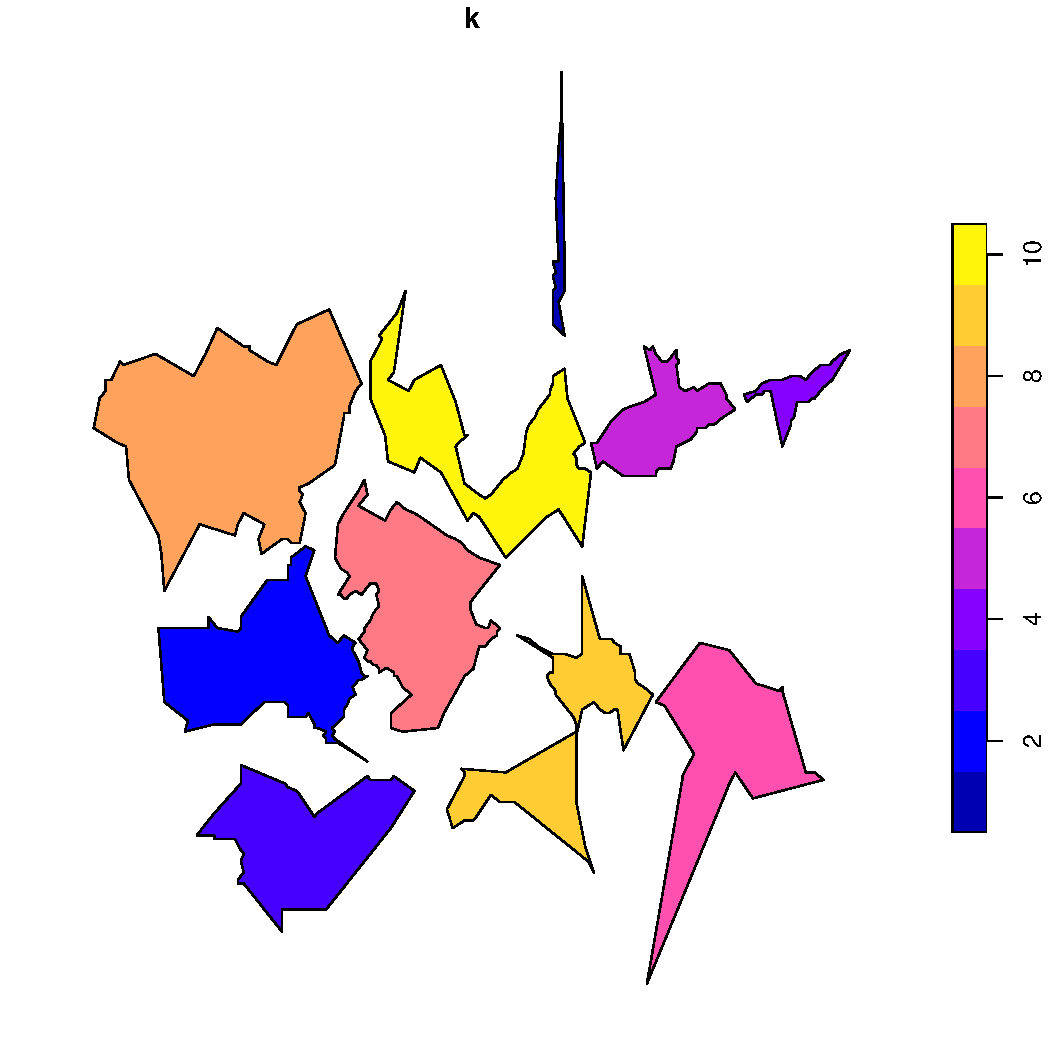
\includegraphics[width=0.9\linewidth]{polygons.pdf}
    \caption{Concave hull of the built-in dataset}
    \label{fig:polygons}
\end{figure}

\section{3D implementation ``\cctd''}

We packaged our implementation as an R package by forking the original repository and replacing JS code with our implementation of the algorithm. The code of the algorithm itself is in TypeScript, compiled and bundled into a single JS file invoked using the \lstinline{V8} package, similarly to the original setup.
Unlike the original package, we initialize the JS evaluation context only once instead of at every function call, and used \lstinline{V8}'s native Foreign Function Interface to perform JS function calls, this makes interoperation more efficient and possibly faster.

\begin{lstlisting}[language=R]
ctx <- V8::v8()
ctx$source(system.file("js", "static", "concaveman3d-bundle.js", package = "concaveman3d"))

interop <- function(points, concavity, length_threshold) {
    ctx$call("concaveman3d.concaveman3dInterop", as.matrix(points), concavity, length_threshold)
}
\end{lstlisting}

Due to the significant differences between the \ccvmn and the the Park-Oh algorithm, we opted to reimplement the 3D variant from scratch.
To compute the convex hull, we used an off-the-shelf 3D implementation of ``quickhull'' \cite{10.1145/235815.235821}.

To keep the retrieval of candidate digging points efficient, we maintain both a hash set of incident faces for each point of the hull, and a hash set of internal points. This way we can easily iterate over just the inner points, and quickly retrieve the faces adjacent to any face. When we analyse a face, we retrieve the faces incident to its three vertices, and merge the sets; this gives all the adjacent faces to a face.

To help demonstrate the algorithm, we included a small web demo \ref{fig:demo}, it is shipped along our package, in the \lstinline{inst/js/static} folder, and can be served by an \lstinline{http} server. It is also available at \url{https://kayjay7.github.io/concaveman3d/}. The demo was used to generate the renders in Figure \ref{fig:caving}.

We offer a toggle to enable distance checks to all faces, as explained in subsection \ref{sub:incorrectness}. This switch is not exposed in the R interface.

\begin{figure}[H]
    \centering
    \includegraphics[width=0.9\linewidth]{demo.png}
    \caption{Screenshot of the web demo}
    \label{fig:demo}
\end{figure}

We also provide a large 3D point cloud as a built-in dataset, generated in the same way as those used in the benchmark. The code is found in \lstinline{data-raw/points3d.R}, and can be imported (after importing the library) using \lstinline{data(points3d)}. In the next subsection we'll give more detail about the point cloud generation method.

\subsection{Performance}

To run the benchmark, we decided to use a function $\mathbb R^2\mapsto\mathbb R$ to generate points in a 3D space with a concave shape:

$$
f\left(x,y\right)=10+\left(\frac{x}{15}\right)^{2}+15\cdot\sin\left(\frac{y}{6}\right)+\left(\frac{y}{20}\right)^{2}
$$

This gives us a surface similar to a curly potato chip, shown in Figure \ref{fig:chip}. The sinusoidal component (the ``curlyness'') helps obtaining Z-thickness once randomness is added to it. We sample the value of the function at regular intervals, add some random noise to each point, and then cull the points that are outside of the inscribed circle, to make the cloud rounder. The result is randomly sampled from this population. Below the R implementation:

\begin{lstlisting}[language=R]
shape <- function(x, y) 10 + (x / 15)^2 + 15 * sin(y / 6) + (y / 20)^2

generation <- function(n) {
    range <- 150
    noise <- 3
    population <- seq(-range, range, length.out = ceiling((sqrt(n)) * 2)) # n^2 - pi(n^2)/4
    population <- expand.grid(x = population, y = population)
    population$z <- shape(population$x, population$y)
    errors <- data.frame(x = rnorm(nrow(population), 0, noise), y = rnorm(nrow(population), 0, 2 * noise), z = rnorm(nrow(population), 0, 5 * noise))
    population <- population + errors
    population <- population[population$x^2 + population$y^2 < range^2, ]
    population[sample.int(nrow(population), n), ]
}

sample <- generation(2000)
\end{lstlisting}

\begin{figure}[H]
    \centering
    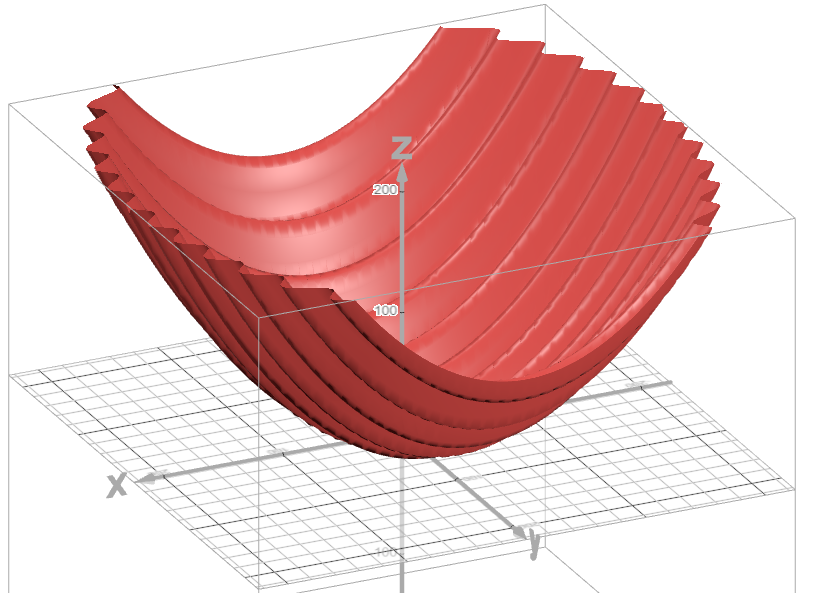
\includegraphics[width=0.8\linewidth]{chip.png}
    \caption{Plot of $f\left(x,y\right)$}
    \label{fig:chip}
\end{figure}

We expect this shape to be a particularly bad case for the algorithm, because the round bottom leads to a more faceted convex hull to iterate on, and at the top, the pronounced, point dense, concavity causes the algorithm to add a large number of additional points to the concave hull. We found \lstinline{concavity = 3.5} and \lstinline{length_threshold = 15} to yield reasonably hard instances.

\bigskip

Before running the benchmark, we ``warm up'' the JavaScript runtime by running the algorithm multiple times on a small dataset. This causes the engine to compile and optimise the hottest code paths, and will give us more consistent results in the following tests.

The runtime of each run is measured using the built-in \lstinline{system.time(output <- algorithm(), gcFirst = TRUE)} function, where the \lstinline{gcFirst} parameter triggers the garbage collector prior to running the expression in order to get more consistent timings. After that, the timings and sizes are stored on a dataframe, and saved to a file for later analysis. Below the snippet running the benchmarks:

\begin{lstlisting}[language=R]
number <- 1
run <- function(x) {
    number <<- number + 1
    sample <- generation(x)
    cat("running", number, "time of", count, "with size:", x, "\n")
    (system.time(hull <- concaveman3d(sample, 3.5, 15), gcFirst = TRUE))[["elapsed"]]
}

count <- 150
low <- 100
hi <- 2000

# warming up the JS engine
p <- generation(200)
for (i in 1:100) concaveman3d(p)


# running benchmark
sizes <- ceiling(seq(low, hi, length.out = count))
times <- unlist(lapply(sizes, run))
sample <- data.frame(sizes = sizes, times = times)

print(sample)

save(sample, file = "thesis/benchmark_data.rda")
\end{lstlisting}

\subsection{Results}

We know that the algorithm's complexity is supposed to be somewhere between quadratic and cubic. The actual time will be random and dependant on the specific arrangement of the points and faces, not just the size of the input. We try to fit both a quadratic and a cubic model and see how well they perform. Neither fully captures the complexity, but we expect them to be a reasonable approximation. In figure \ref{fig:benchmark} we compare the fitted lines against a plot of the data:

\begin{figure}[H]
    \centering
    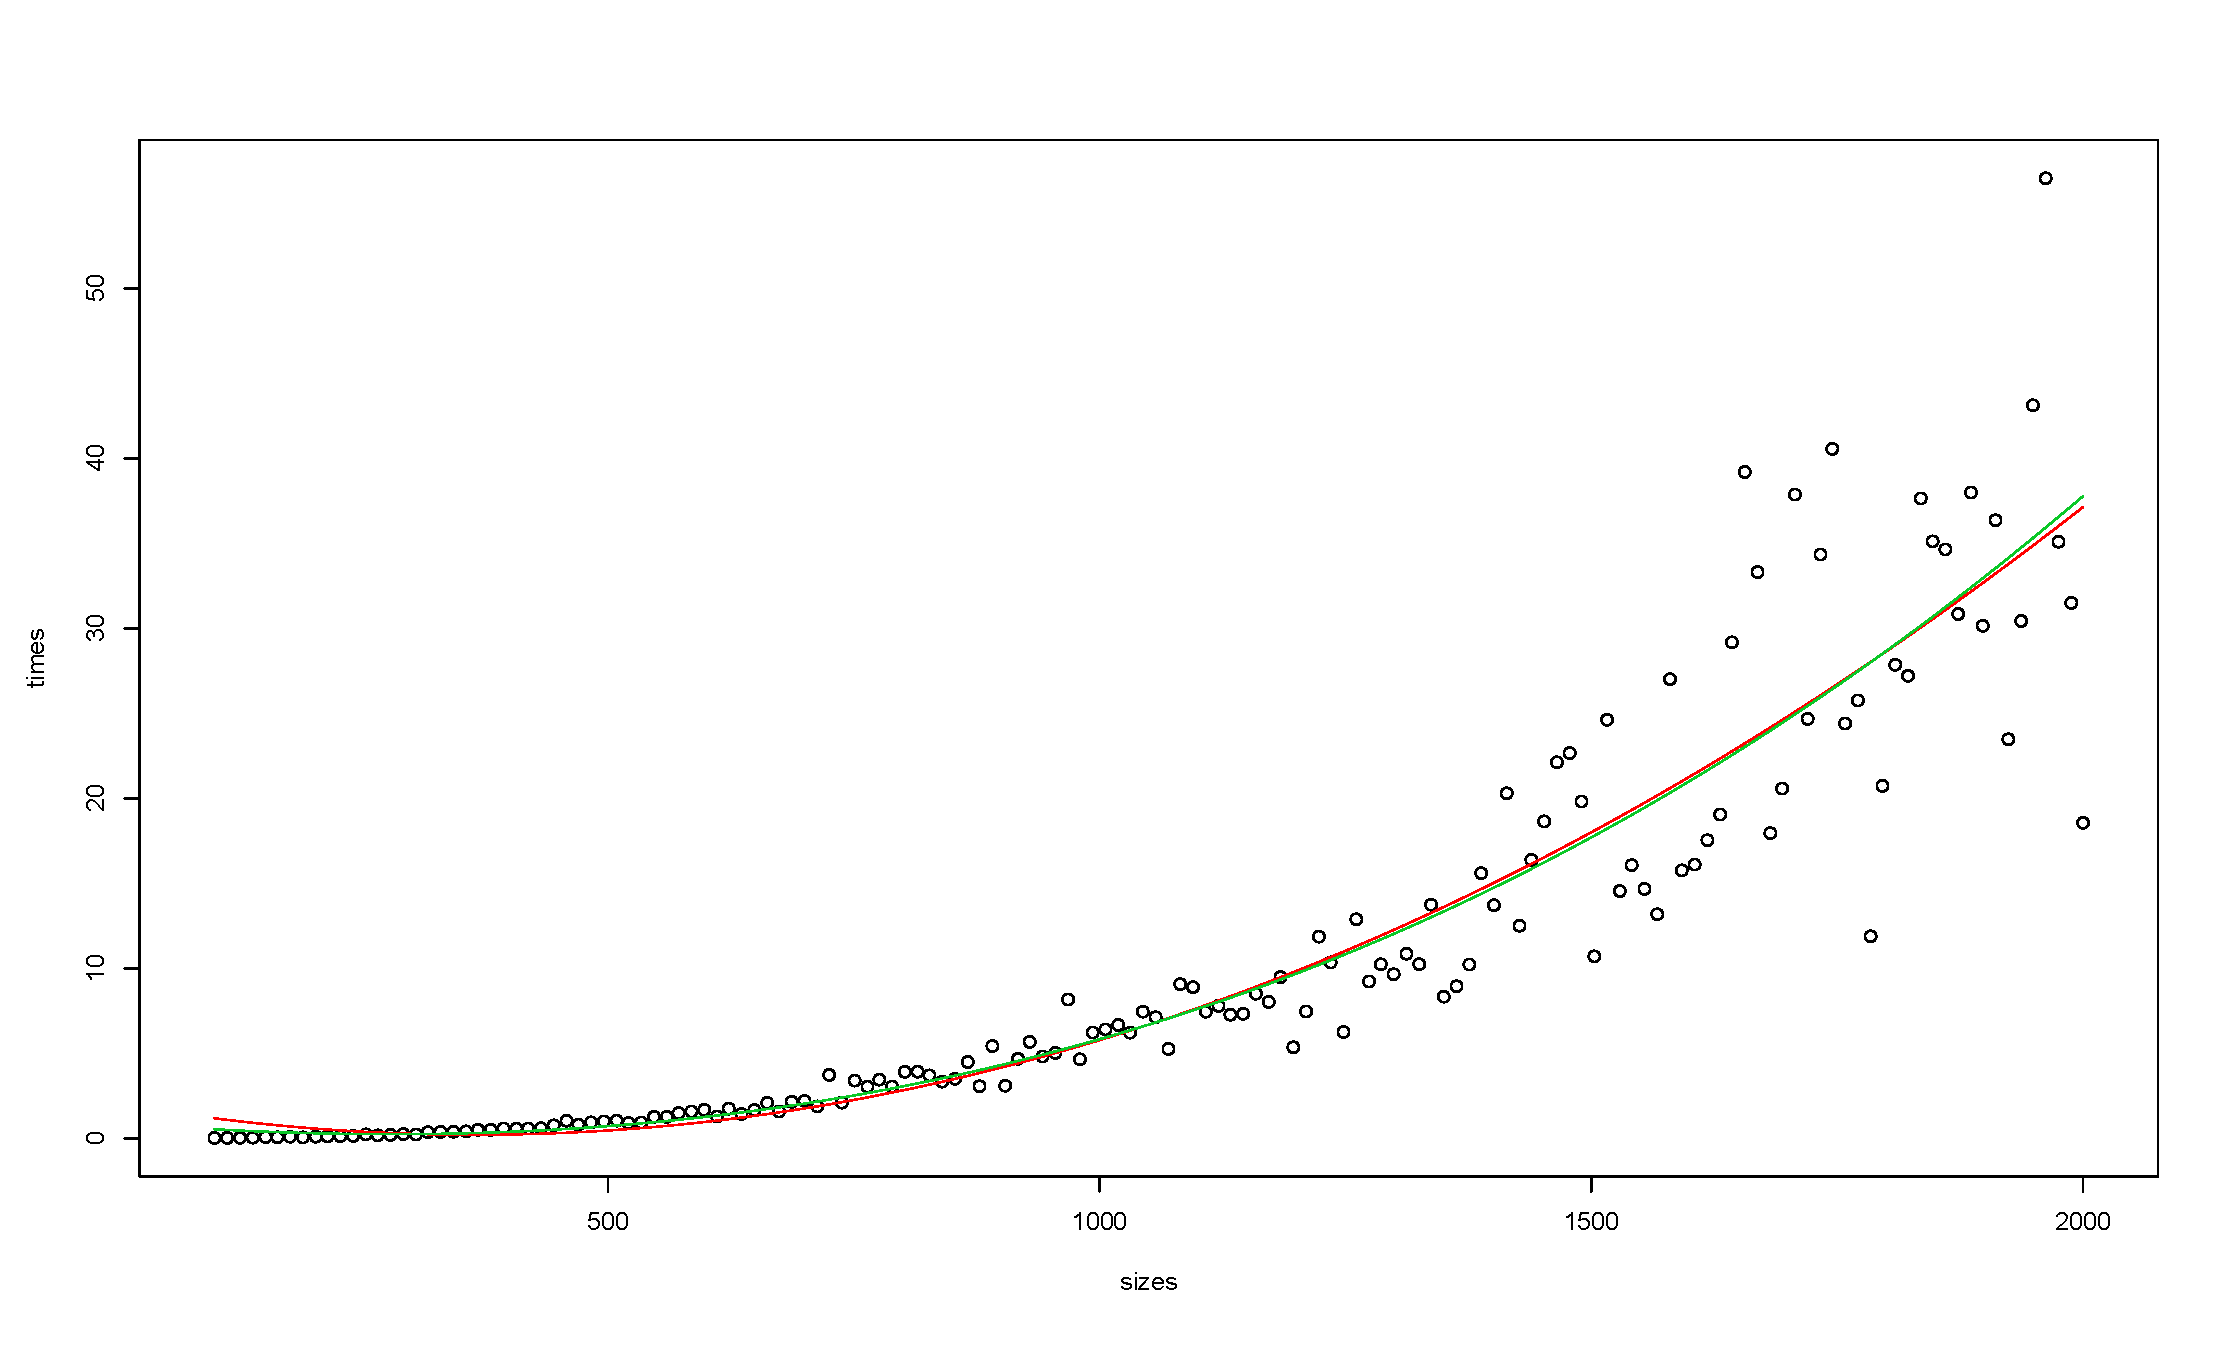
\includegraphics[width=1\linewidth]{benchmark.eps}
    \caption{Scatterplot of the benchmark results (in black), the fitted quadratic curve (in red), and the fitted cubic curve (in green)}
    \label{fig:benchmark}
\end{figure}

At a glance, we can see that both models follow the sample, but as the input size get larger, the behaviour becomes more erratic (less predictable). Unsurprisingly, there is little observable difference between the quadratic and cubic curves. The P-values are both approximately $0$, and the R-squared values are both around $0.85$, these values are good, but the plotted summaries in Figure \ref{fig:quadratic} and Figure \ref{fig:cubic} are less positive:

\begin{figure}[H]
    \centering
    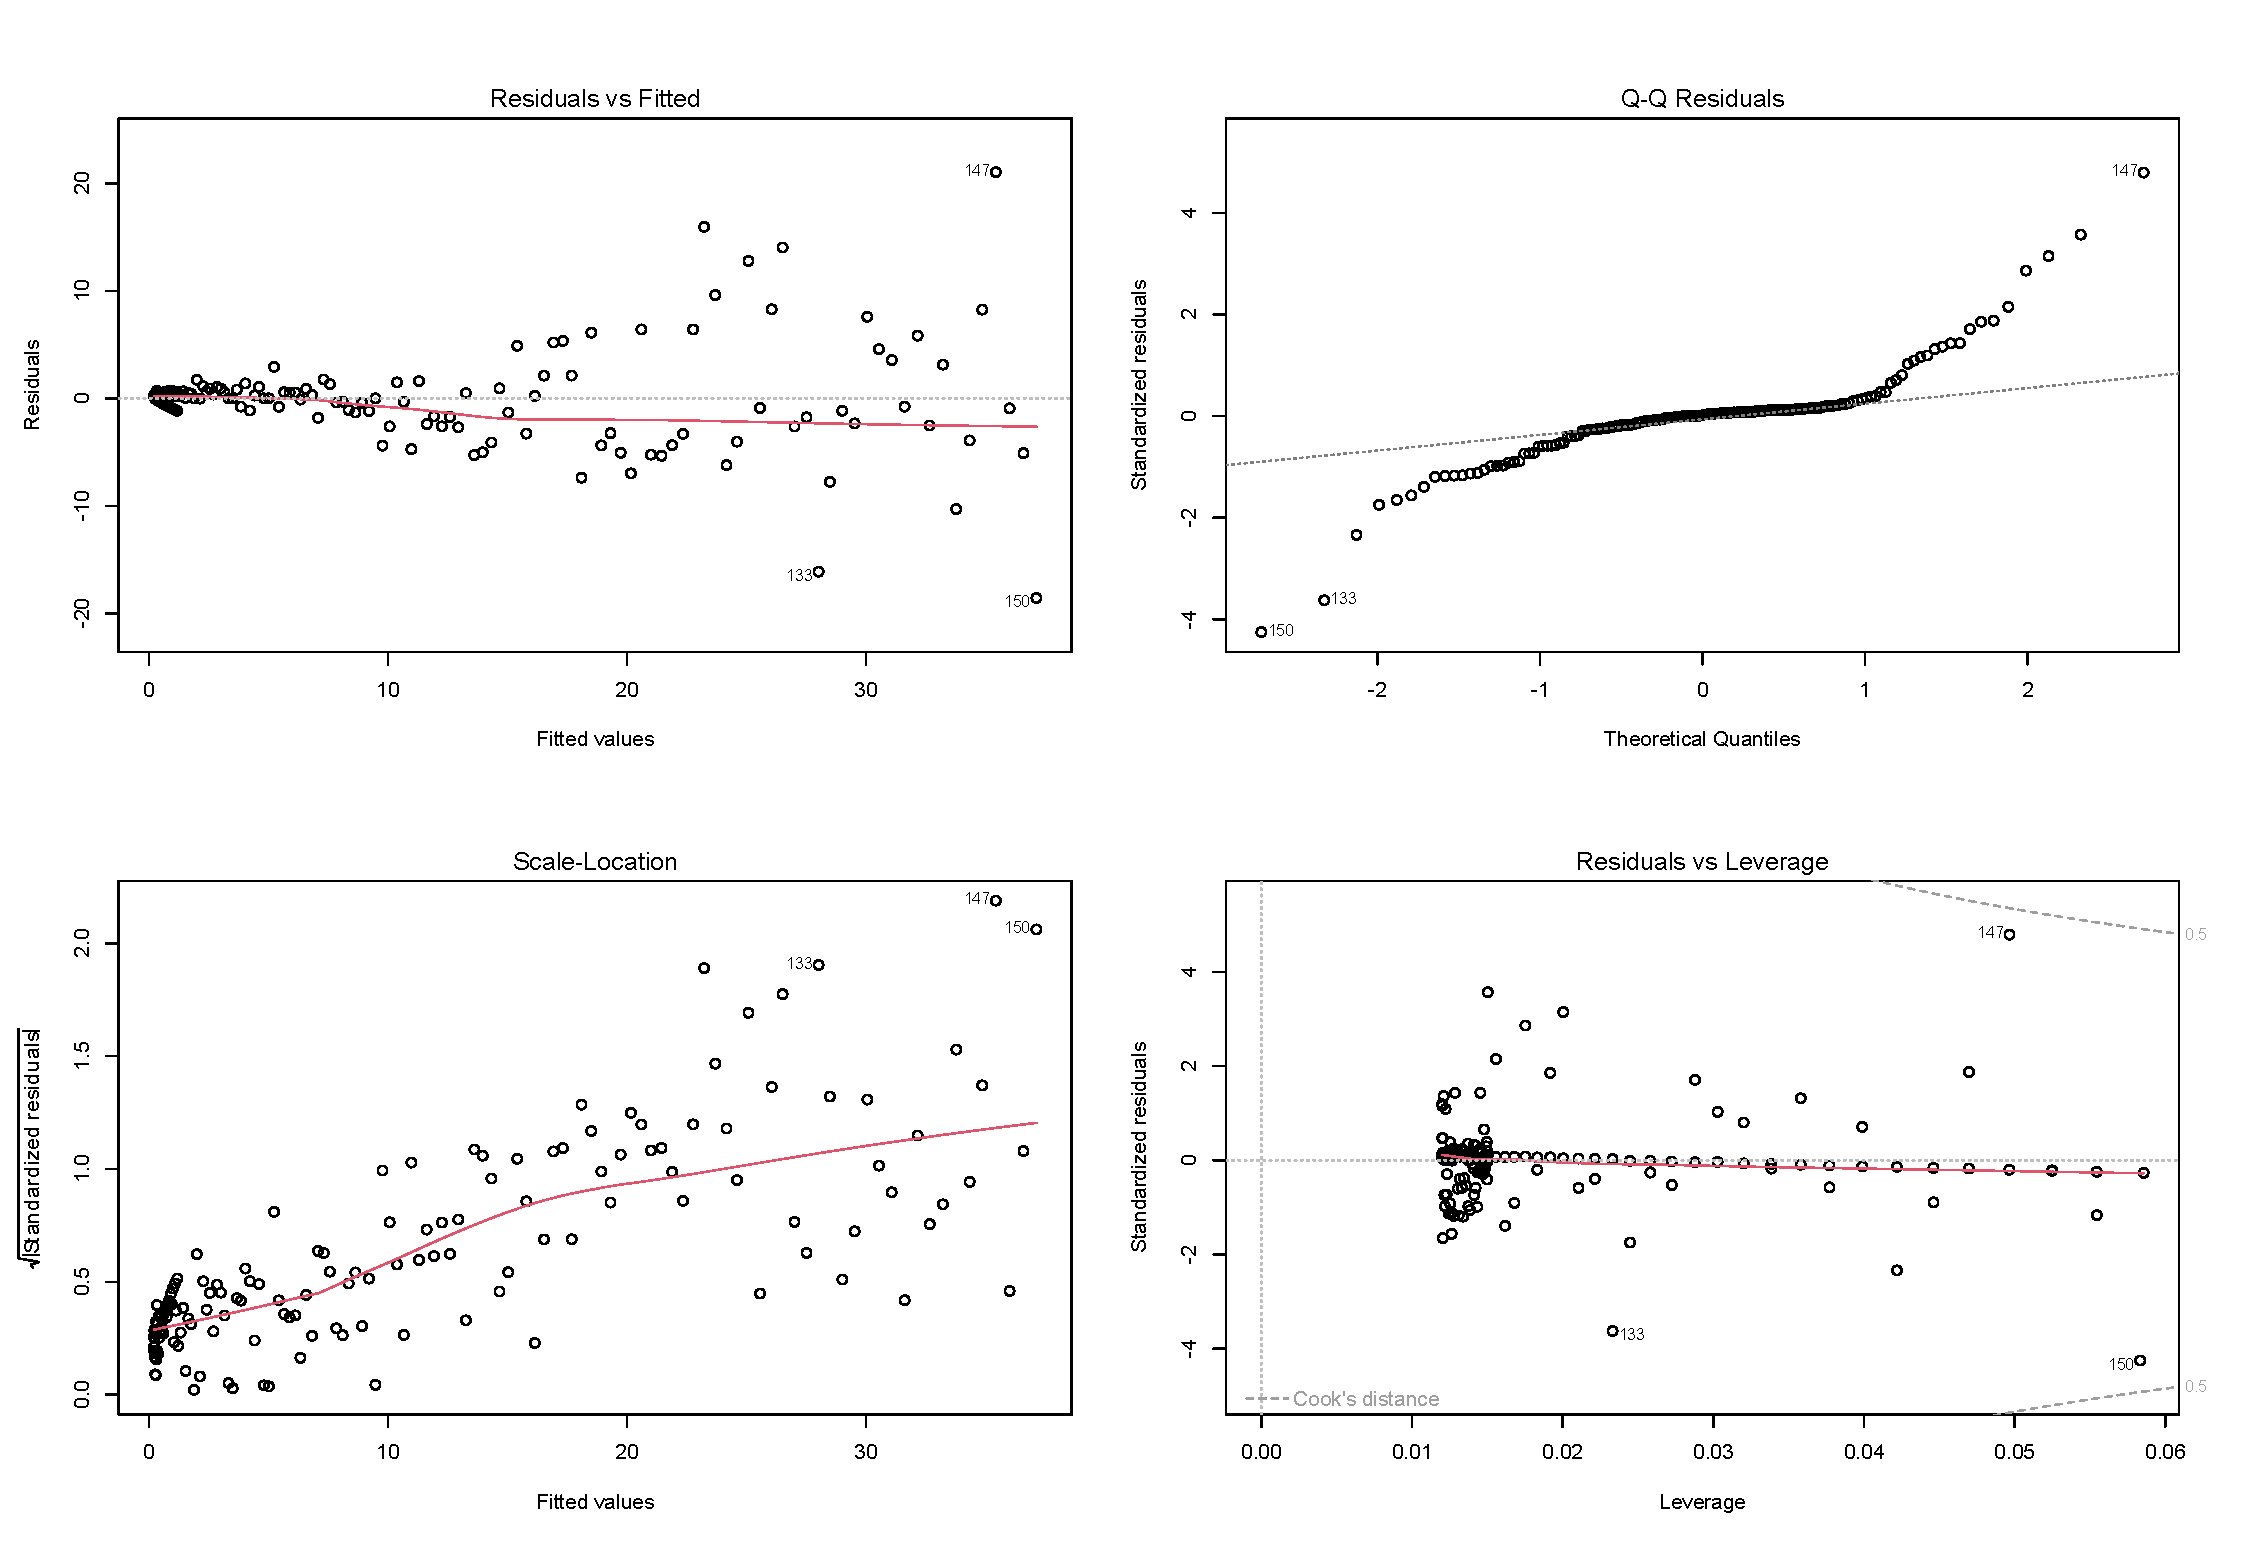
\includegraphics[width=1\linewidth]{benchmark-summary-2.eps}
    \caption{Summary plots of the quadratic model}
    \label{fig:quadratic}
\end{figure}

\begin{figure}[H]
    \centering
    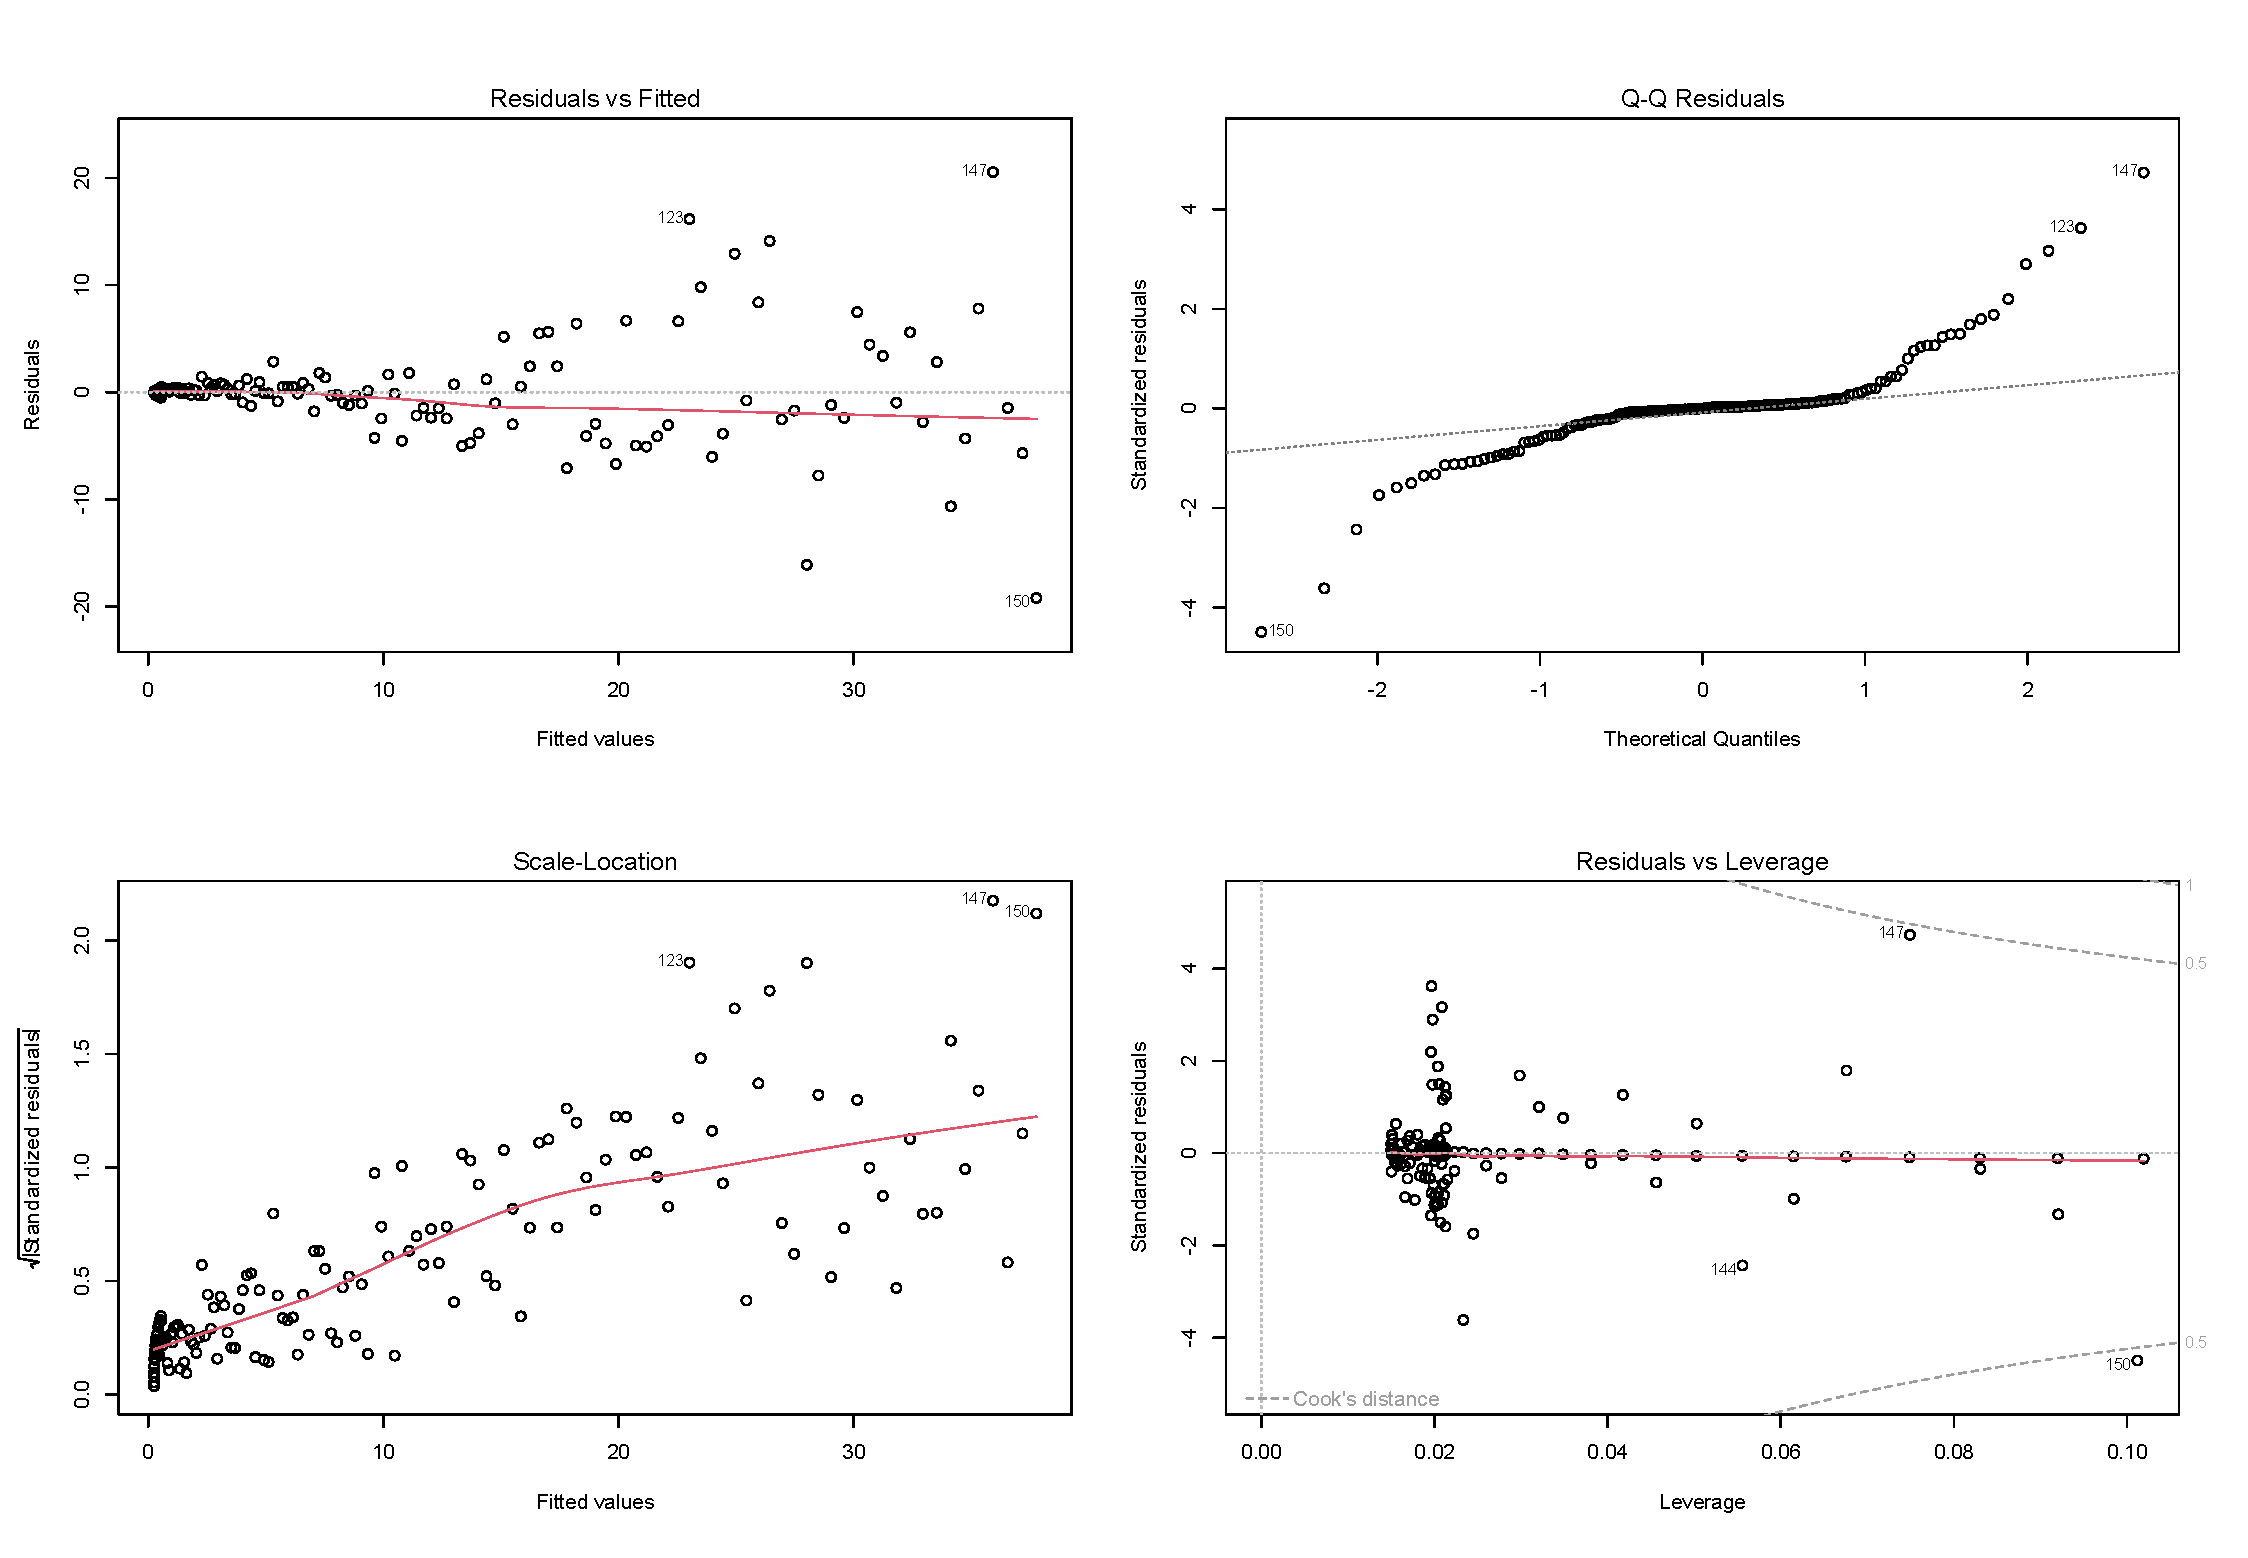
\includegraphics[width=1\linewidth]{benchmark-summary-3.eps}
    \caption{Summary plots of the cubic model}
    \label{fig:cubic}
\end{figure}

In both cases, the ``residuals vs fitted'' plot is decent, although it shows some clustering on the lower values. The other plots show signs of divergence from the model.

These results are in line with our understanding of the algorithm in that the models do follow the data, but since the real cost of the computation depends also on uncontrollable parameters, neither model can be expected to perform particularly well.

\section{Bibliography}
\bibliographystyle{alpha}
\bibliography{sample}

\end{document}
